\documentclass[12pt, a4paper]{report}
\usepackage[utf8]{inputenc}
%\usepackage[T1]{fontenc}
\usepackage[czech]{babel}
\usepackage{amsmath}

\usepackage{listings}
\usepackage{svg}
\usepackage{graphicx}
\graphicspath{ {./images/} }

\title{KIV/PC\\Zadání č.3\\Hledání Minimální Kostry Grafu\\Jiří Veselý}
\begin{document}
\maketitle
\tableofcontents

%
% Zadání
%
\chapter{Zadání}
Detailní znění zadání je na stránce\\ https://www.kiv.zcu.cz/studies/predmety/pc/doc/work/sw2020-03.pdf
%
% Rozepisování analýzy
%
\chapter{Analýza úlohy}
\section{Rozbor}
Úlohu lze rozdělit do tří částí. Prvním krokem je načtení dat ze souborů hran a vrcholů. Druhou částí spuštění kruskalova algoritmu na hledání minimální kostry grafu. Poslední částí je export nalezených hran do daného souboru, podle zadaného parametru -mst nebo -mrn. Úloha vede k řešení pomocídatové struktury ohodnoceného neorientovaného grafu.
%
% Ohodnocený neorientovaný graf
%
\subsection{Ohodnocený neorientovaný graf}
Ohodnocený neorientovaný graf se chápe jako množina vrcholů a hran. Hrany definují spojení mezi jednotlivými vrcholy a cenu tohoto spojení. Na směru hrany nezáleží. Například, pokud je hrana mezi vrcholy 1 a 2, tak je i hrana mezi vrcholy 2 a 1.
\begin{figure}[h!]
\centering
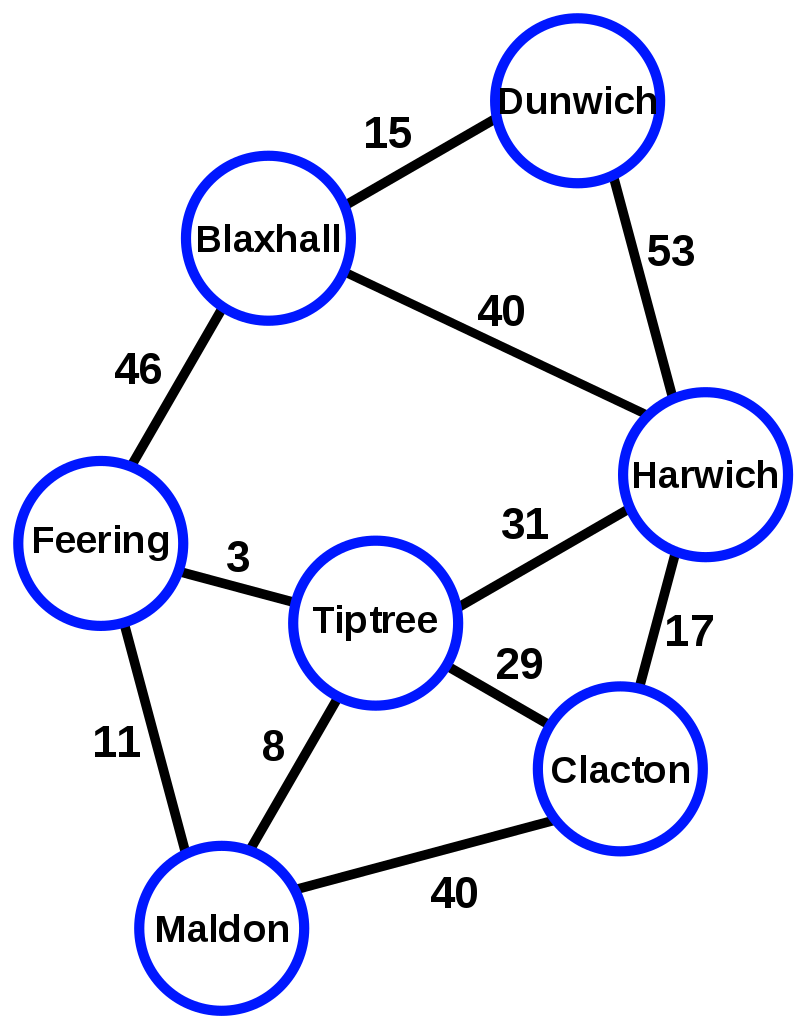
\includegraphics[width=3cm, height=4cm]{graph_example}
\caption{Příklad Ohodnoceného Neorientovaného grafu}
\end{figure}
%
% ADT Graf
%
\newpage
\subsection{Reprezentace datové struktury Graf}
Pro řešení datové struktury Graf existují dvě nejčastější řešení. První využívá datovou strukturu Spojový seznam a druhá využívá Matici souslednosti.
%
% Matice sousednosti
%
\subsubsection{Matice Sousednosti}
Matice sousednosti je matice \emph{A} definována, jako NxN matice, kde N reprezentuje počet vrcholů. Indexy \emph{i} a \emph{j} v reprezentují vrcholy, tudíž pro: $A_{ij} = x$, \emph{x} může být libovolný znak a reprezentuje hranu z vrcholu \emph{i} do \emph{j}. Tento znak u ohodnoceného grafu reprezentuje cenu této hrany.
\\ \\
Implementace tohoto řešení není složitá, neboť spočívá ve vytvoření dvourozměrného pole o rozměrech NxN, kde N reprezentuje počet vrcholů. Zásadním problémeme tohoto řešení je jeho paměťová neefektivita a náročnost. V datech poskytnutých pro tuto úlohu je přibližně 26000 validních vrcholů a 28000 validních hran. To znamená, že by bylo \emph{$((26000)^2-28000)$} nevyužitých prvků.
\begin{equation}
A = \begin{bmatrix} 
    a_{11}   & 0 & a_{13} & \dots &  a_{1K}  \\
    \vdots   &  \ddots &  \dots  & \dots & \vdots\\
   \vdots   &  \ddots &  \dots  & \dots & \vdots\\
    a_{K1}   & 0 & \dots     & a_{KK-1}   & 0 
    \end{bmatrix}
\end{equation}
Výhoda matice sousednosti, je rychlý přístup k prvku se složitostí \emph{O(1)}. Takže toto řešení by bylo vhodné pro malé grafy. Pro data, která byla spokytnutá k této úloze je toto řešení velice nevhodné.
\end{figure}
%
% Spojový seznam
%
\newpage
\subsubsection{Spojový seznam}
Narozdíl od matice sousednosti, \emph{Spojový seznam}, neplýtvá pamětí na nepoužité prvky. Spojový seznam je struktura, která obsahuje atribut, ve kterém je uložen odkaz na další prvek seznamu, tím vzniká spojení (hrana).\\\\
Použití spojového seznamu je velmi vhodné na použití poskytnutých dat, protože by spojení vrcholů a hran je řídké. Pokud by matice souslednosti byla plně zaplněná, nemá smysl používat spojový seznam, protože paměťová náročnost by byla stejná, ale vypočetní náročnost větší.
%
%
%
\chapter{Popis implementace}
Data ze souboru se ukládají do pole struktur hran a vrcholů. Před jejich vložením do polí se filtrují podle pokynů v zadání. Implementace Kruskalova algoritmu se provadí pomocí spojového seznamu. Původně jsem chtěl použít řešení pomocí matice souslednosti, ale kvůli paměťové náročnosti jsem od tohoto řešení upustil.\\\\
Implementace je pomocí 4 knihoven a ty jsou \emph{edge}, \emph{vertex}, \emph{graph} a \emph{usefc}.
\section{Přehled}
%
% edge
%
\subsection{edge.h}
První knihovna je \emph{edge}. Jak už název napovídá, jedná se o strukturu, která obsahuje atributy hrany.
\begin{lstlisting}[language=C]
edge *edge_load(const char filename[], uint *datasize);
int edge_compar_fn_by_id(const void *p1, const void *p2);
int edge_compar_fn_by_clen(const void *p1, const void *p2);
int edge_compar_fn_by_id_down(const void *p1, const void *p2);
int edge_compar_fn_by_clen_down(const void *p1, const void *p2);
void edge_print(edge *edge_data, uint datasize);
void edge_export_mst(edge *edge_data, uint datasize, char *filename);
void edge_export_mrn(edge *edge_data, uint datasize, char *filename);
\end{lstlisting}
\pagebreak
%
% vertex
%
\subsection{vertex.h}
Další knihovnou je \emph{vertex}. Tato knihovna je velmi podobná knihovně \emph{edge}, ale řeší uložení vrcholů.
\begin{lstlisting}[language=C]
vertex *vertex_load(const char filename[], uint *datasize);
int vertex_compar_fn(const void *p1, const void *p2);
void vertex_print(vertex *vertex_data, uint datasize);
int vertex_get_key_by_id(vertex *vertex_data, uint datasize, uint id);
\end{lstlisting}
%
% graph
%
\subsection{graph.h}
Další knihovnou je \emph{graph}. Tato knihovna je zajišťuje vytvoření grafu a řeší kruskalův algoritmus.
\begin{lstlisting}[language=C]
graph* createGraph(uint vertex_dlen, uint edge_dlen, edge *edges);
uint find(subset subsets[], uint i);
void Union(subset subsets[], int x, int y);
edge* KruskalMST(graph* graph_temp, vertex *vertex_data,
uint *edge_mst_len);
\end{lstlisting}
%
% usefc
%
\subsection{usefc.h}
Další knihovnou je \emph{usefc}. Tato knihovna obashuje užitečné funkce, které se hodili při řešení úlohy.
\begin{lstlisting}[language=C]
void printArrayString(int size, char **values);
int inArrayString(int size, char **values, char *search);
\end{lstlisting}

\newpage
\section{Rozbor funkcí}
V této sekci budou vysvětleny dané funkce a jejich účel.
%
%
%
% edge
%
\subsection{edge}
%
%
%
\subsubsection{edge\_load}
Tato funkce načte data ze souboru hran a vytvoří pole struktur hran. Při načítání se řeší filtrování podle pokynů v zadání. Nejprve se ověří hlavička souboru hran. Poté se připravý paměť pro hranu na aktuálním indexu. Dalším krokem je vykopírování atributu WKT z řádky souboru, aby se mohla řádka dále rozdělit podle znaku ','. Pokud se má daná hrana ignorovat, nezvýší se index uvolní se paměť pro atribut WKT. Fuknce vratí pointer na první index v poli hran.
%
%
%
\subsubsection{edge\_compar\_fn\_by\_id}
Tato funkce slouží k porovnání dvou prvků podle id. Používá se pro seřazení hran podle id vzestupně.
%
%
%
\subsubsection{edge\_compar\_fn\_by\_clen}
Tato funkce slouží k porovnání dvou prvků podle clen. Používá se pro seřazení hran podle id sestupně.
%
%
%
\subsubsection{edge\_compar\_fn\_by\_id\_down}
Tato funkce slouží k porovnání dvou prvků podle id. Používá se pro seřazení hran podle id vzestupně.
%
%
%
\subsubsection{edge\_compar\_fn\_by\_clen\_down}
Tato funkce slouží k porovnání dvou prvků podle clen. Používá se pro seřazení hran podle id sestupně.
%
%
%
\subsubsection{edge\_print}
Vypíše obsah předaného pole hran.
%
%
%
\subsubsection{edge\_export\_mst}
Exportuje hrany do souboru podle argumentu -mst.
%
%
%
\subsubsection{edge\_export\_mrn}
Exportuje hrany do souboru podle argumentu -mrn.
%
%
%
% vertex
%
\subsection{vertex}
%
%
%
\subsubsection{vertex\_load}
Obdobná funkce jako funkce edge\_load akorát, že načte vrcholy.
%
%
%
\subsubsection{vertex\_compar\_fn}
Porovnávací fuknce vrcholů podle jejich id. Slouží k seřazení vrcholů podle id vzestupně.
%
%
%
\subsubsection{vertex\_print}
Tato fuknce vypíše obsah předaného pole vrcholů.
%
%
%
\subsubsection{vertex\_get\_key\_by\_id}
Funkce vratí na jakém indexu se nachází vrchol v poli vrcholů s předaným atributem id. Pokud není nalezen, vrátí -1.
%
%
%
% vertex
%
\subsection{graph}
%
%
%
\subsubsection{createGraph}
Funkce vytvoří strukturu graph a načte do ní předané hrany.
%
%
%
\subsubsection{find}
Rekurzivně projde předané pole subsets a vratí root prvek prvku i.
%
%
%
\subsubsection{Union}
Zajišťuje spojení hran, které jsou navíc. Slouží k imlementaci kruskalova algoritmu.
%
%
%
\subsubsection{KruskalMST}
Funkce vrátí pole struktur hran. Tyto hrany tvoří minimální kostru grafu.
%
%
%
% vertex
%
\subsection{usefc}
%
%
%
\subsubsection{printArrayString}
Tato funkce vypíše obsah pole stringů.
%
%
%
\subsubsection{inArrayString}
Vrátí id, kde se nachází hledaný prvek. Pokud pole prvek neobsahuje, vratí -1.
%
%
%
\section{main}
Ještě zbývá funkce main, která je vstupním bodem aplikace. Funkce nejprve ošetří argumenty z příkazové řádky. Poté načte vrcholy, hrany a seředí je podle id vzestupně. Toto seřezení není nutné, ale pro lepší orientaci v datech jsem jej implementoval.Pokud zadané argumenty říkají, že se má řešit minimální kostra, tak se spustí kruskalův algoritmus a exportuje nalezené hrany do požadovaných souborů. Pokud se minimální kostra řešit nemá, program skončí s návratovou hodnotou \emph{EXIT\_SUCCESS}. Posledním krokem je uvolnění alokované paměti.
%
%
%
%
%
\chapter{Uživatelská příručka}
Pro přeložení projektu je třeba spustit soubor Makefile. Za předpokladu absence fatálních chyb se tímto projekt přeloží a vytvoří se spustitelný soubor graph. 
\section{Spuštění programu}
Program očekává dva povinné parametry následované souborem obsahující data. Prvním je -v, tento argument říká, že dalším argumentem je datový soubor vrcholů. Druhým je -e, tento argument říká, že dalším argumentem je datový soubor hran.\\
Následují dva nepovinné argumenty. Prvním je -mst. Tento argument říká, že program má ze zadaných dat vytvořit minimální kostru grafu a uložit ji do souboru definovaným v následujícím argumentu. Druhým je -mrn. Tento argument říká, že program má ze zadaných dat vytvořit minimální kostru grafu a uložit ji do souboru definovaným v následujícím argumentu. Formát uložení dat se liší v seřezení a atributech nation, cntryname (viz. zadání).
\chapter{Závěr}
Myslím, že jsem nalezl optimální řešení danné úlohy. Ovšem musím konstatovat, že program by mohl být více optimalizovaný. Například implementace dynamického alokování paměti pro výsledné hrany minimální kostry nebo volbou mezi použitím spojového seznamu a matice souslednoti na základě vstupních dat.\\
Práce je nahraná ve službě github.com na adrese \\https://github.com/teamSPSE/PCsemestralGraph. \\Práce je bohužel soukromá, aby nemohlo dojít k případnému plagiátu. Pro zpřístupnění stačí napsat mail s údaji na veselyj@students.zcu.cz
\end{document}